\documentclass[10pt]{article}
\usepackage[margin=2.2cm]{geometry}
\usepackage{booktabs,graphicx,xcolor,amsmath,amssymb}
\usepackage[hidelinks]{hyperref}
\usepackage{caption}
\captionsetup{font=small,labelfont=bf}
\newcommand{\hw}[1]{\textbf{#1}}

\title{\vspace{-1.2em}Throughput Is Not Learning: Final Report on the Async-Rollout
8B Campaign\\ \large 2$\times$ wall-clock validated; per-sample parity at best; transfer
deficits traced to answer-coverage collapse}
\author{CA-benchmark rung-3 / 8B thread}
\date{2026-08-14}

\begin{document}
\maketitle
\vspace{-2em}

\begin{abstract}
We complete the four-arm 8B campaign crossing two rollout engines (old lockstep vs.\ a
trajectory-concurrent async collector) with two credit-assignment methods (token-GRPO,
turn-PPO) on ASearcher search-RL, 75 steps each, plus a 7{,}152-question transfer
evaluation under three scorers. The async engine's systems claims hold: \hw{2.01$\times$}
end-to-end at matched config, 3--4$\times$ on the rollout phase, zombie generation
49.6\%$\rightarrow$0. Per training \emph{step} it learns $\sim$2$\times$ faster early (val
0.43 vs.\ 0.23 at step 25) --- but sample-matched curves show this is a \emph{data-rate}
effect: at equal cumulative released trajectories the old engine matches or beats it, and
on transfer the old arms win everywhere (macro judge: old turn-PPO \hw{0.550}, old GRPO
0.535, async GRPO 0.506, async turn-PPO 0.445). Decomposition localizes the async deficits
almost entirely to \emph{answer coverage}: conditional on answering, async turn-PPO is the
most accurate arm in the campaign (judge 0.623), but it emits no answer on 30.2\% of
questions (old: 0.3\%), terminating via context exhaustion after long searches; async GRPO
shows the same drift at 1/3 strength. Stale-group drops were zero in both engines ---
staleness censoring is \emph{not} a mechanism. We flag the critic $\times$
partial-rollout-resume interaction as the prime suspect for the late-training regression
(val 0.486$\rightarrow$0.404 over steps 50--75) and recommend a staleness correction plus
answer-commitment shaping before the async engine becomes the training default.
\end{abstract}

\section*{Setup}
Qwen3-8B-Base, unfiltered ASearcher Base-35k, 32-turn horizon, 16k prompt / 1024 response,
top-5 wiki-18/e5 retrieval, 75 steps, both engines with identical partial-rollout config
(cycle 8 / max\_age 4). Async arms (\texttt{async75kv60}): one coroutine per trajectory over
vLLM~V1 AsyncLLM engines, uid-atomic group release, gpu\_util 0.60, sticky routing. Transfer
evaluation: greedy \texttt{val\_only} on the 10-benchmark suite; 7 wiki-answerable
benchmarks (6{,}115~q) reported separately from 3 live-web benchmarks (1{,}027~q, corpus
gap); scorers: strict EM (the training reward), substring EM, gpt-oss-120b judge (frozen
MBE prompt). All four arms evaluated on the same frozen old-engine harness. Caveats:
async-arm evals ran on A100 (old on H100), cross-arch greedy drift $\le$0.02 --- deficits
are 3--8$\times$ that; judge $\approx$ EM$+$0.13, one-directional.

\section{Engine mechanisms (matched profile, corrected)}
\begin{table}[h]\centering\small
\begin{tabular}{lrrr}\toprule
metric & sync & async & ratio\\\midrule
phase wall-clock (3 steps + val + ckpt) & 8{,}953 s & 4{,}454 s & \hw{2.01$\times$}\\
rollout generation, 3-step total & 4{,}890 s & 1{,}228 s & $\sim$3--4$\times$\\
zombie generated tokens & 49.6\% & \hw{0} & ---\\
released trajectories & 2{,}300 & 2{,}695 & 1.17$\times$\\
val@3 (greedy, 512 q) & 0.264 & 0.244 & within $\pm$0.02 band\\\bottomrule
\end{tabular}
\caption{Matched H100 A/B (same config/seed/data). Steady state @0.65 util: 6{,}473 gen
tok/s, 174 traj/min. B200 measured 0.88$\times$ H100 on rollout (TRITON\_ATTN decode
1.6$\times$ slower/token) --- H100 remains the rollout node.}
\end{table}

\hw{Correction:} \texttt{max\_age} stale-group drops were \hw{zero} in both engines across
all 75 steps of all four arms --- stale censoring explains nothing. The operative data-side
differences: (1)~\hw{release volume}: async releases 1{,}200--1{,}700 traj/step vs.\
690--1{,}150 (cumulative 92--94k vs.\ 55--69k), because the old engine's fixed batch
geometry drops surplus completed groups; (2)~\hw{completion mix}: continuous slot backfill
keeps long trajectories that lockstep cycles would truncate or never collect;
(3)~\hw{fresher resumes}: paused trajectories resume immediately rather than at the next
8-turn cycle; (4)~fp16 engine numerics (token ids byte-exact by construction).

\section{Per-step vs.\ per-sample learning}
\begin{figure}[h]\centering
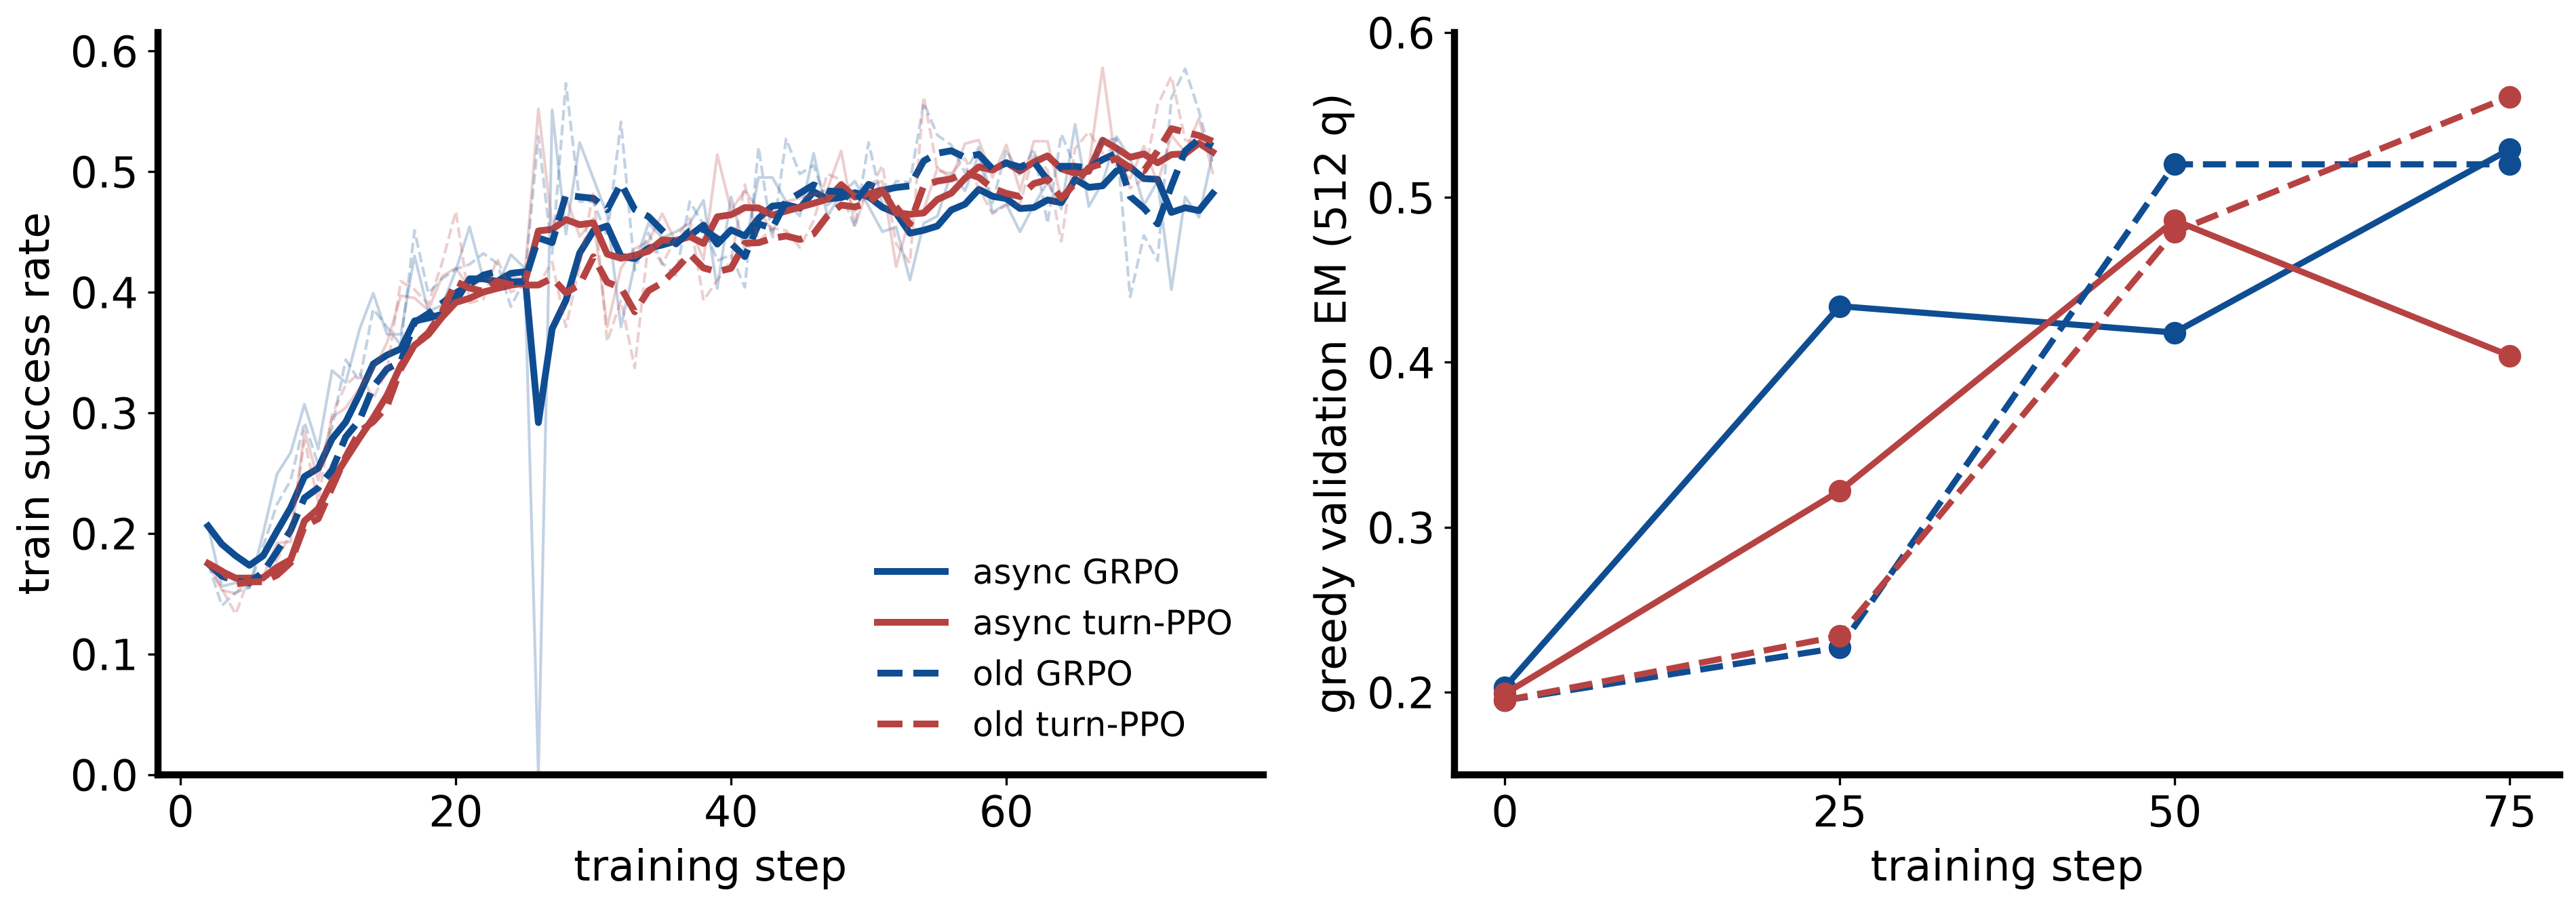
\includegraphics[width=\linewidth]{assets/fig_train_val.png}
\caption{Train success rate (EMA; faint = raw) and greedy val EM by \emph{step}. Async
arms are $\sim$2$\times$ ahead at step 25. Dips near step 26 are pod-reclaim/OOM resume
replays, not learning events.}
\end{figure}
\begin{figure}[h]\centering
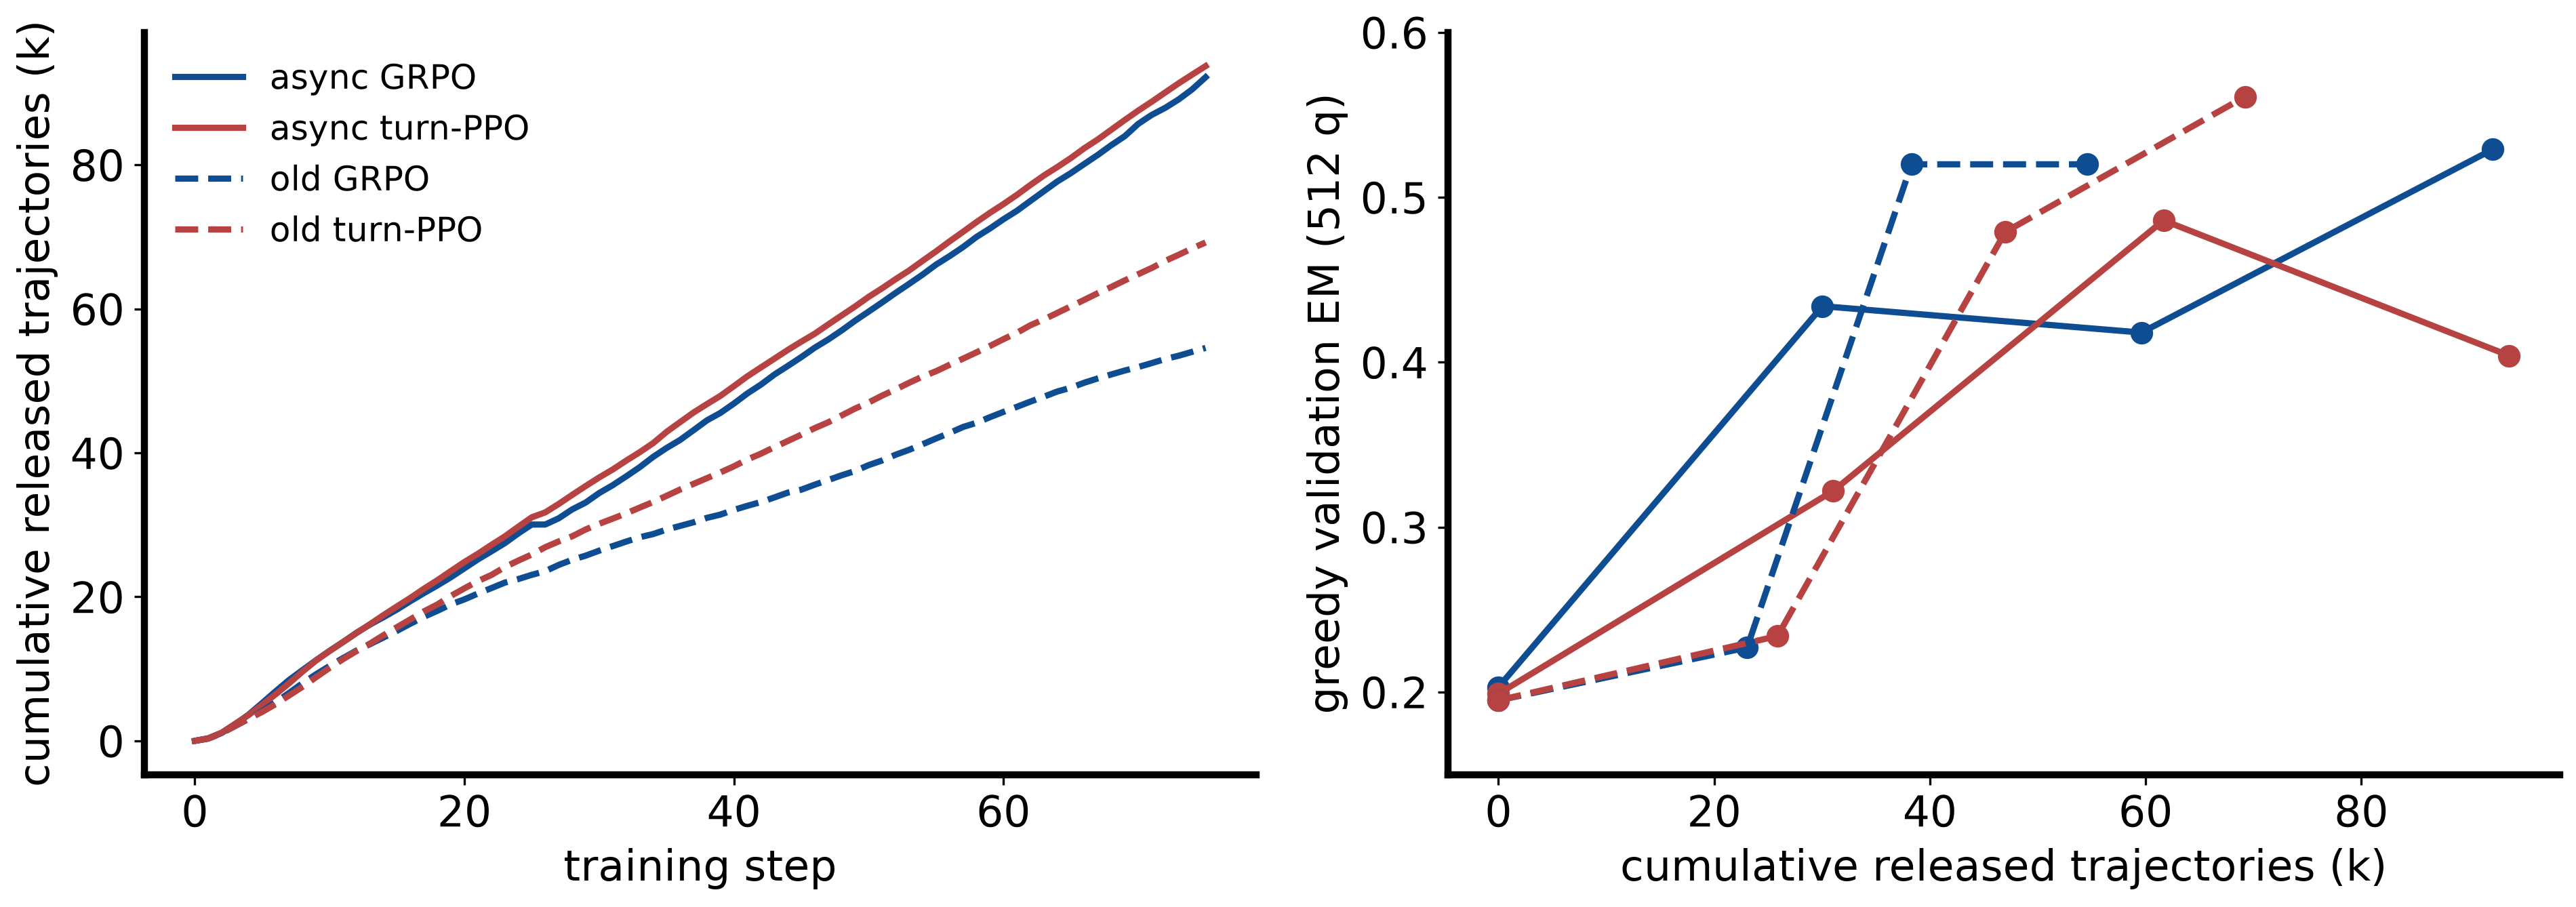
\includegraphics[width=\linewidth]{assets/fig_sample_matched.png}
\caption{The same val points re-indexed by cumulative released trajectories. The async
per-step advantage is a data-rate effect: old GRPO reaches 0.520 by $\sim$38k
trajectories; async GRPO needs $\sim$92k for 0.529. Async turn-PPO peaks at 0.486 (61k)
then \emph{falls} to 0.404 (94k).}
\end{figure}

\begin{table}[h]\centering\small
\begin{tabular}{llrrrr}\toprule
arm & engine & val@0 & val@25 & val@50 & val@75\\\midrule
old GRPO & lockstep & 0.195 & 0.227 & 0.520 & 0.520\\
old turn-PPO & lockstep & 0.195 & 0.234 & 0.479 & \hw{0.561}\\
async GRPO & async & 0.203 & 0.434 & 0.418 & 0.529\\
async turn-PPO & async & 0.199 & 0.322 & 0.486 & 0.404\\\bottomrule
\end{tabular}
\caption{Greedy strict-EM validation (512 q, $\pm$0.02 reproducibility).}
\end{table}

\section{Transfer: the ordering reverses}
\begin{figure}[h]\centering
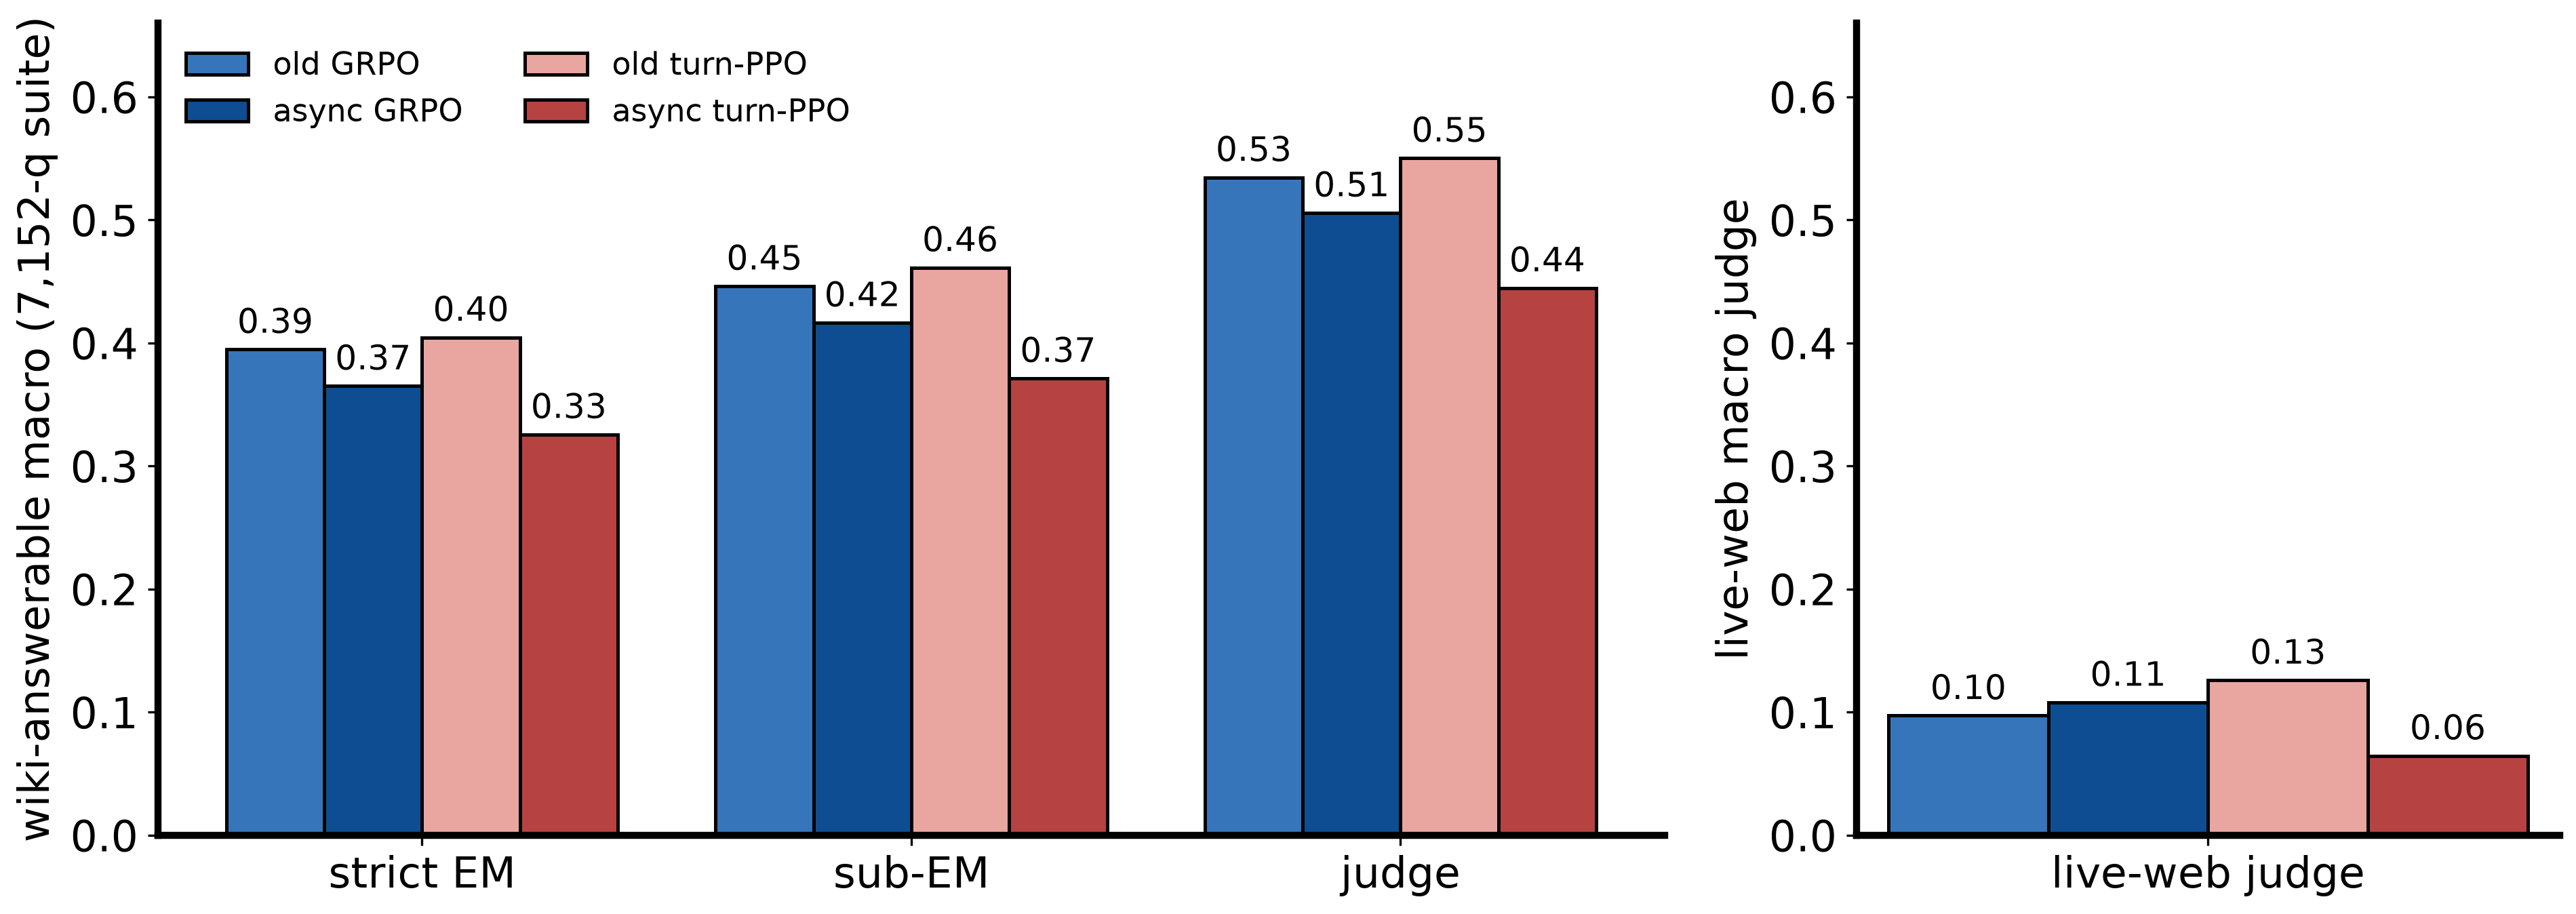
\includegraphics[width=\linewidth]{assets/fig_transfer_4way.png}
\caption{Wiki-answerable macro under three scorers, plus live-web judge. Old engine wins
every cell; the async GRPO train-val advantage (0.529 vs.\ 0.520) reverses on transfer
(0.506 vs.\ 0.535).}
\end{figure}

\section{Failure analysis: answer coverage, not accuracy}
\begin{table}[h]\centering\small
\begin{tabular}{lrrrrr}\toprule
arm & judge (all) & judge (answered) & no-answer & mean turns & median\\\midrule
old GRPO & 0.535 & 0.571 & 6.2\% & 17.5 & 18\\
async GRPO & 0.506 & 0.573 & 11.7\% & 18.7 & 19\\
old turn-PPO & 0.551 & 0.552 & 0.3\% & 7.8 & 3\\
async turn-PPO & 0.435 & \hw{0.623} & \hw{30.2\%} & 8.5 & 3\\\bottomrule
\end{tabular}
\caption{Wiki-answerable decomposition. Conditional accuracy is preserved or improved
under the async engine; coverage is what collapses.}
\end{table}
\begin{figure}[h]\centering
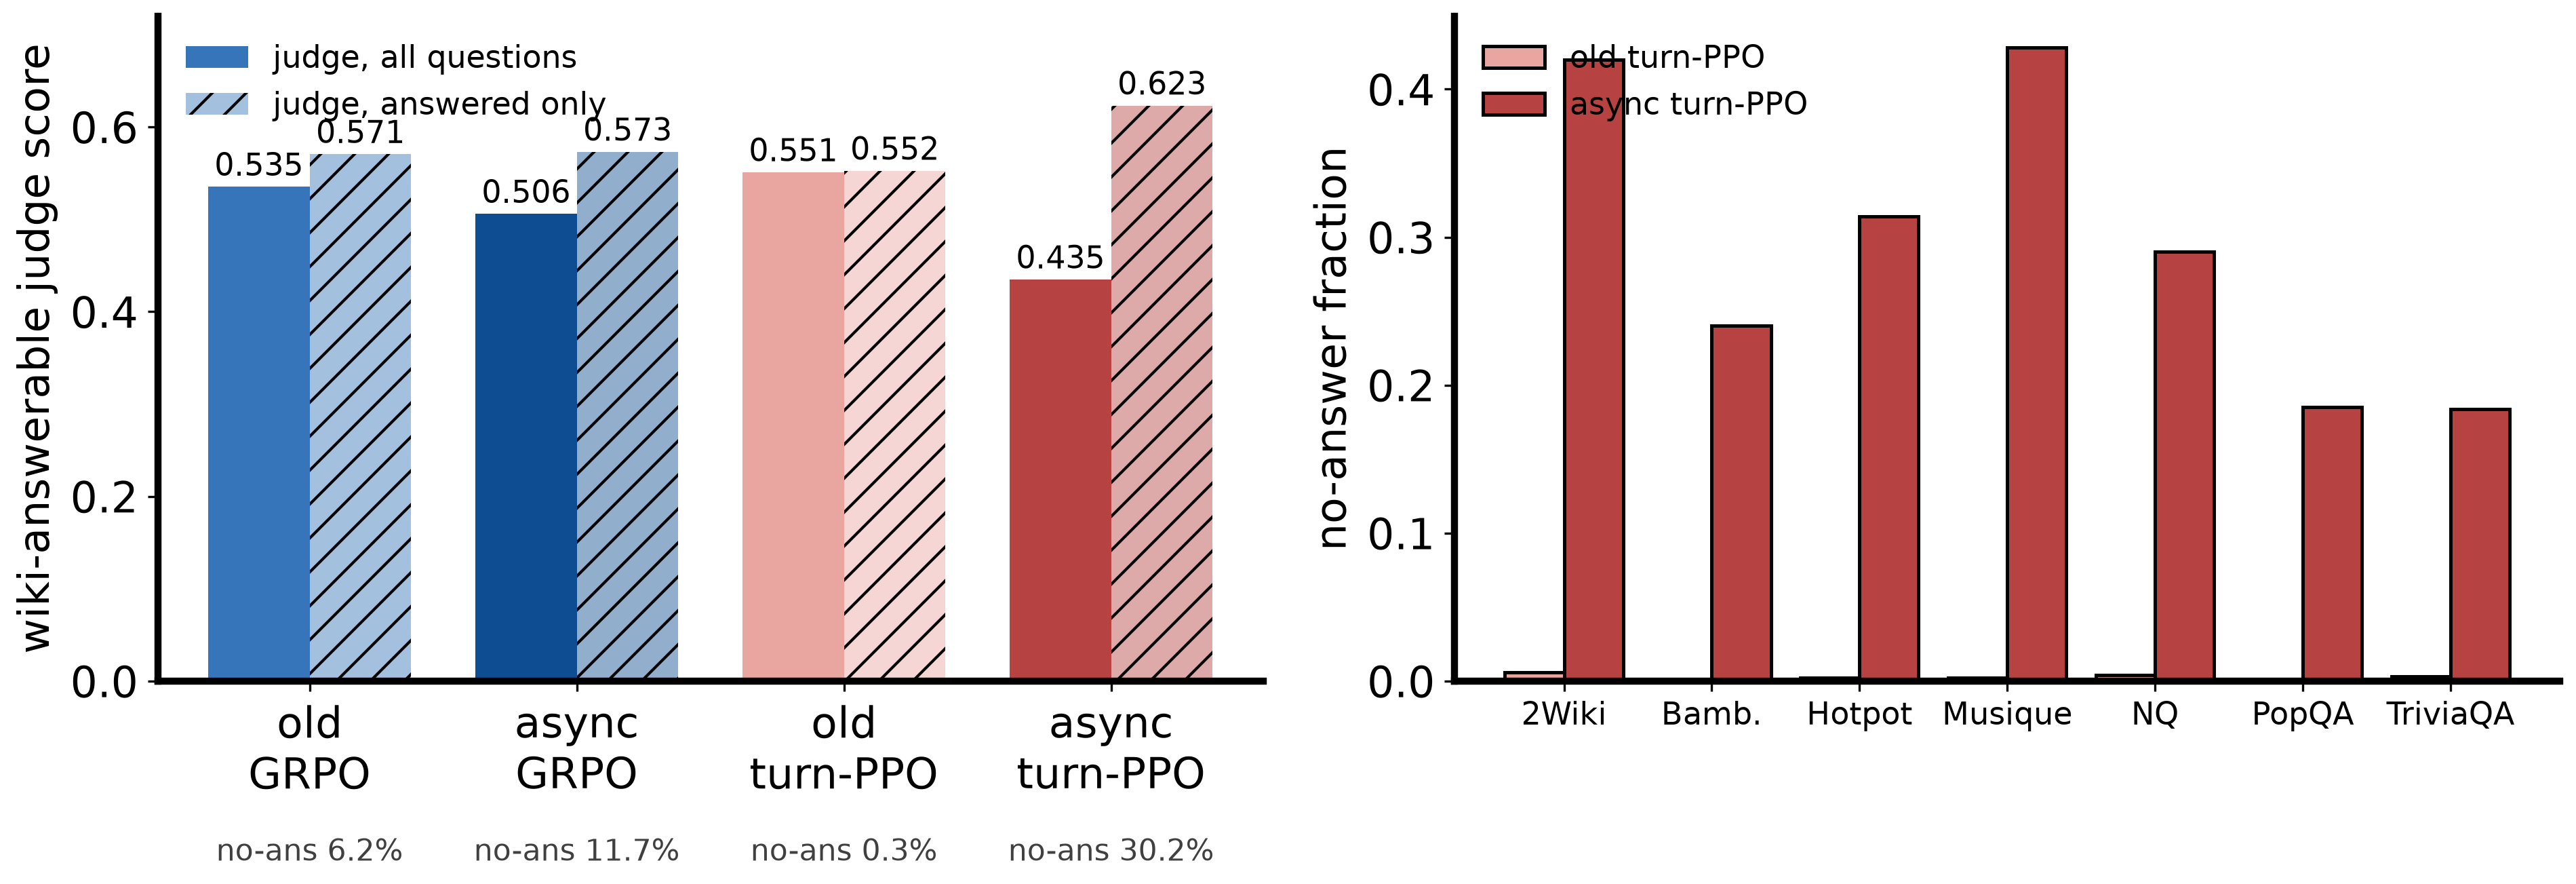
\includegraphics[width=\linewidth]{assets/fig_noanswer.png}
\caption{Left: all-question vs.\ answered-only judge score. Right: async turn-PPO
no-answer concentrates on multihop benchmarks (Musique 43\%, 2Wiki 42\%, Hotpot 31\%).}
\end{figure}
\begin{figure}[h]\centering

\includegraphics[width=0.72\linewidth]{assets/fig_turns_dist.png}
\caption{Turn distributions (wiki-answerable). Both turn-PPOs are bimodal (52--54\% answer
within 3 turns); async shifts the search mode right. Async GRPO inflates the 20--23 bucket
to 35\% (old: 10\%). No arm hits the 32-turn cap.}
\end{figure}

Paired per-question analysis (async vs.\ old turn-PPO, 6{,}116 common questions): 1{,}028
lost, 318 gained; \hw{720 of the 1{,}028 losses are no-answer terminations}. No-answer
trajectories average 17.2 turns with \hw{0\%} at the 32-turn cap: they end by
\emph{context exhaustion} (\texttt{ctx\_terminate}) --- the policy searches until the 16k
window fills without committing to an answer. The drift is training-time: async turn-PPO's
own val fell 0.486$\rightarrow$0.404 (steps 50--75) while train success kept rising. Prime
suspect: the \hw{critic $\times$ partial-rollout-resume interaction} --- resumed
trajectories carry returns realized under older policies; a turn-level critic bootstraps
across the resume seam, and async's higher resume volume makes the value of ``continue
searching'' systematically stale-optimistic. GRPO (no critic) shows the same direction at
$\sim$1/3 strength. Candidate fixes: behavior-IS staleness correction (parked item R2),
answer-commitment shaping, resume-age cap for critic arms.

\section{Credit-assignment sweep (old engine, 5 estimators)}
\begin{table}[h]\centering\small
\begin{tabular}{llrrrr}\toprule
estimator & mechanism & val@0 & val@25 & val@50 & val@75\\\midrule
GRPO & token-level group-relative & 0.195 & 0.227 & 0.520 & 0.520\\
turn-PPO (b0) & turn-level GAE + critic & 0.195 & 0.234 & 0.479 & \hw{0.561}\\
token-PPO & stock token GAE + critic & 0.195 & \hw{0.312} & \emph{pending} & \emph{pending}\\
HCAPO & hindsight answer-cond., $\gamma{=}0.95$ & 0.195 & 0.297 & \emph{pending} & \emph{pending}\\
GiGPO & anchor-state + episode groups & 0.195 & 0.064 & \emph{pending} & \emph{pending}\\\bottomrule
\end{tabular}
\caption{Estimator comparison on the lockstep engine (\texttt{fast75}). token-PPO / HCAPO /
GiGPO died with their pods at steps 42/44/46 and were resumed 2026-08-14 from step 25 on
identical code; \emph{pending} cells fill as the resumed runs reach steps 50/75.}
\end{table}
\begin{figure}[h]\centering
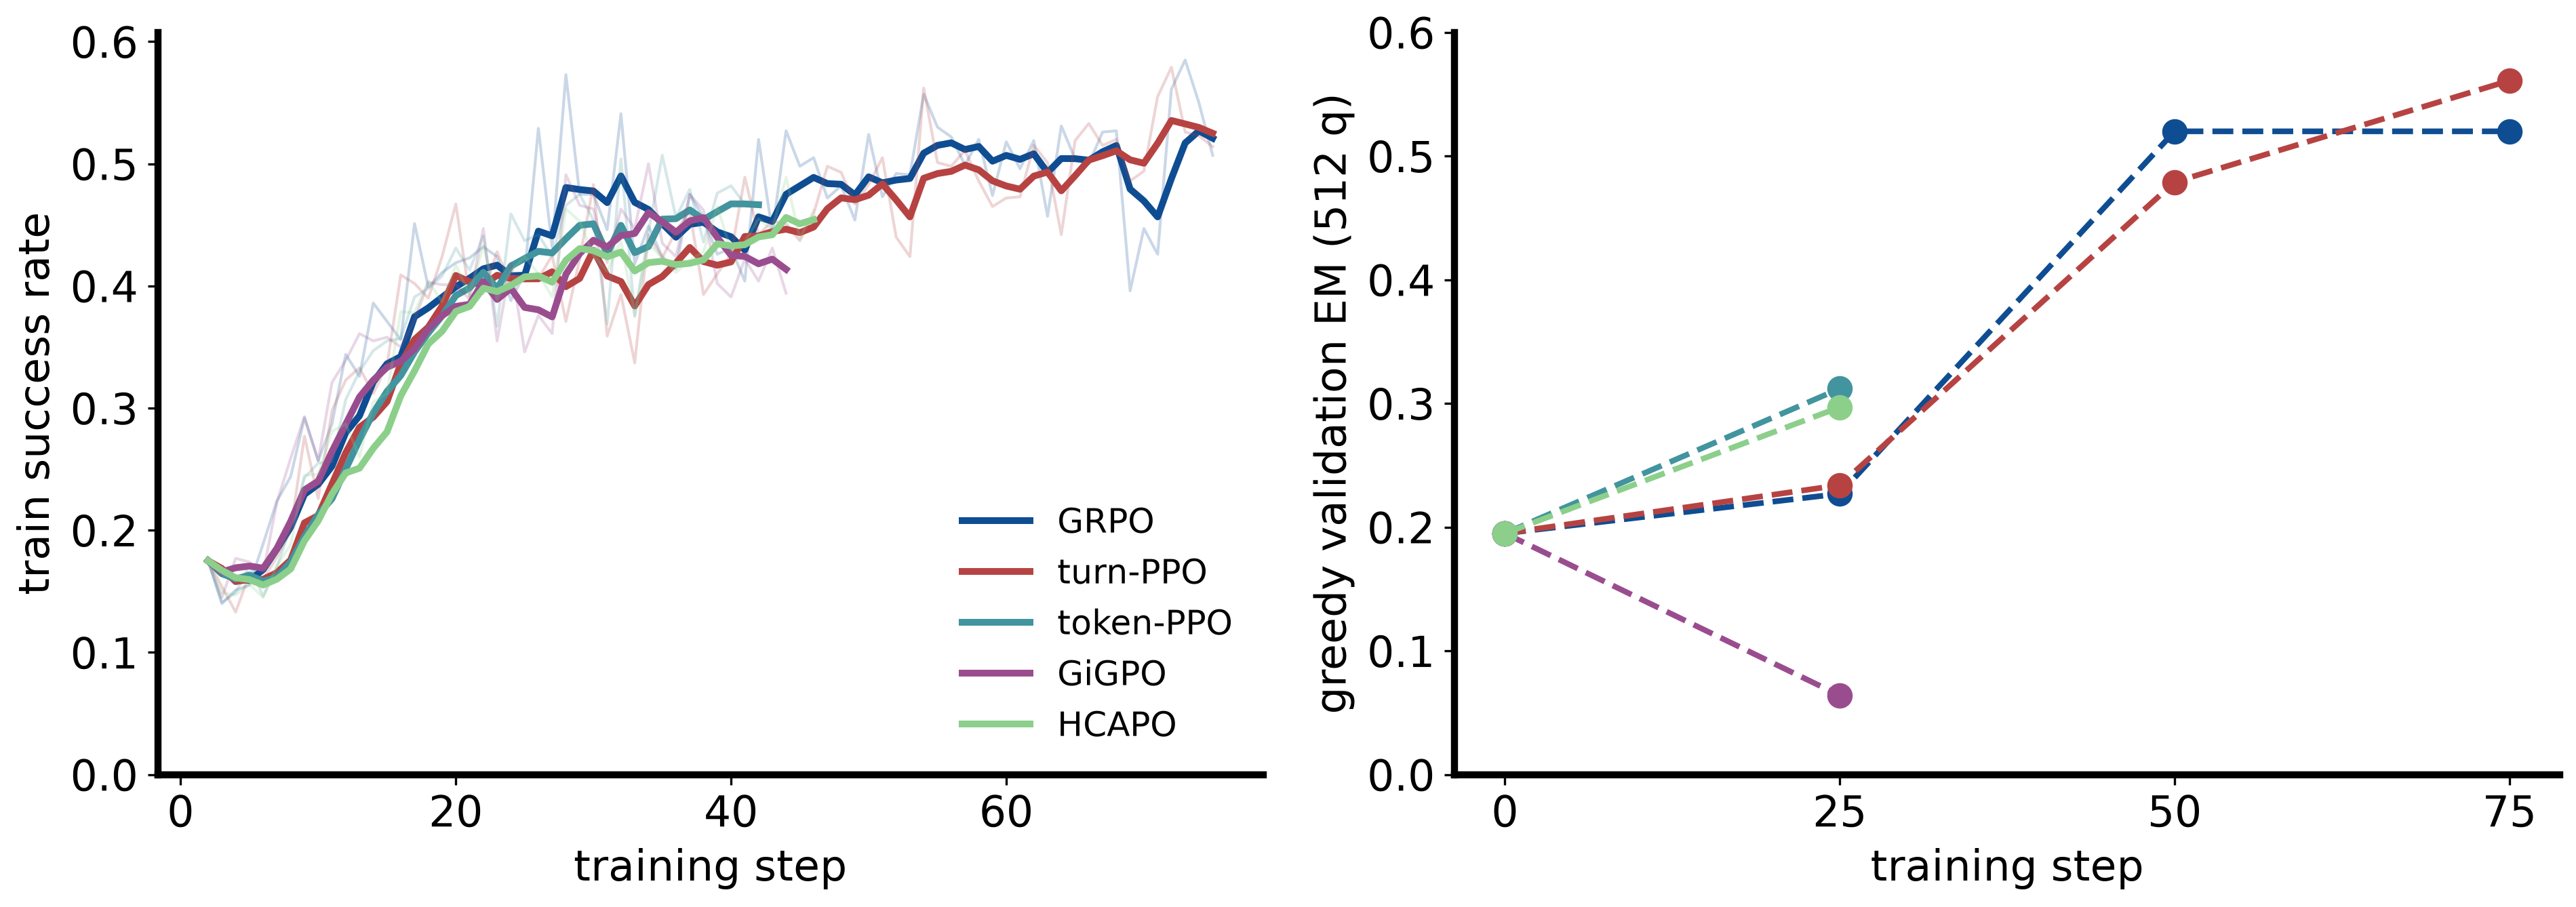
\includegraphics[width=\linewidth]{assets/fig_estimators.png}
\caption{Five-estimator training curves. token-PPO (0.312) and HCAPO (0.297) lead at step
25 --- ahead of where the two finished arms stood (0.227/0.234), though those finished at
0.52/0.56, so val@25 is weakly predictive. \hw{GiGPO's val collapsed (0.064) while its
train success stayed normal ($\sim$0.45)} --- a train/val divergence, not a failed run.
HCAPO's $\gamma{=}0.95$ is a deliberate protocol deviation (paper value).}
\end{figure}

\section*{Verdict}
Adopt the async collector for what it is: a \hw{2$\times$ wall-clock engine} with clean
semantics (atomic groups, zero zombie generation, val parity at profile scale). Do not yet
adopt it as the training default: its data distribution (more, longer, fresher-resumed
trajectories) pushes policies toward non-committal search, mildly for GRPO and severely for
critic-based turn-PPO. Fix order: (1) staleness/IS correction at the resume seam,
(2) answer-commitment shaping or no-answer penalty, (3) re-run the turn-PPO arm; the
sample-matched curves here are the baseline any fix must beat.
\end{document}
